\documentclass[a4paper]{article}

\usepackage[english]{babel}
\usepackage{amsmath}
\usepackage{amssymb}
\usepackage{dsfont}
\usepackage{tikz}
\usepackage{framed} 
\usetikzlibrary{arrows,automata}
\title{Calculus and Probability Theory\\ Assignment 5}
\author{Christoph Schmidl\\
s4226887\\
Informatica\\
c.schmidl@student.ru.nl\\}
\date{\today}


\begin{document}
\maketitle





\textbf{After completing these exercises successfully you should be confident with the following topics:}

\begin{itemize}
	\item familiar with definite and indefinite integrals
	\item able to apply the most important integration methods, more specifically, substitution and integration
	\item confident about switching between different representations of a function
	\item able to compute area of a finite or infinite region
	\item able to apply the formula for the arc length of a function over a finite interval
\end{itemize}
\vspace{1em}

\begin{enumerate}


%%%%%%%%%%%% Task 1 %%%%%%%%%%%%
\item (\textbf{20 points}) Compute the following indefinite integrals. You can use \textit{substitution} or \textit{integration by parts}. In each problem \textit{verify} your result, and don't forget about the constant term. You may need some of the following, well-known trigonometric identities:

\begin{align}
	\sin(2x) = 2\sin(x)\cos(x), \quad \cos(2x) = \cos^2(x) - \sin^2(x), \quad \sin^2(x) + \cos^2(x) = 1\notag
\end{align}

Also, it is highly recommended to consult with the lecture slides and solve the problems there before you start with these ones.

\begin{enumerate}
	%%%%%%%% Task 1.a %%%%%%%%
	\item $\int \sin(x) \cos(x) \; dx$\\
	\textbf{Solution:}\\
	
\begin{align}
	u &= \sin(x)\notag\\
	du &= \cos(x) dx\notag\\
	dx &= \frac{du}{\cos(x)}\notag
\end{align}	
	
	
\begin{align}
	\int \sin(x) \cos(x) \; dx &= \int u \cos(x) \frac{du}{\cos(x)}\notag\\
	&= \int u \; du\notag\\
	&= \frac{1}{2}u^2\notag\\
	&= \frac{1}{2} \sin^2(x) + C\notag
\end{align}	
	
	
	%%%%%%%% Task 1.b %%%%%%%%
	\item $\int \ln(ax) \; dx$ where $a > 0$\\
	\textbf{Solution:}\\
	
Using integration by parts = $\int f' \cdot g = f \cdot g - \int f \cdot g'$\\	
	
	
\begin{align}
	g &= \ln(ax)\notag\\
	g' &= \frac{1}{x}\notag\\
	f &= x\notag\\
	f' &= 1\notag
\end{align}	
	
	
\begin{align}
	\int \ln(ax) \; dx &= x \cdot \ln(ax) - \int x \cdot \frac{1}{x}\notag\\
	&= x \cdot \ln(ax) - \int 1\notag\\
	&= x \cdot \ln(ax) - x + C\notag
\end{align}		
	
	%%%%%%%% Task 1.c %%%%%%%%
	\item $\int \cos^2(x) \; dx$\\
	\textbf{Solution:}\\

\begin{align}
	\int \cos^2(x) \; dx &= \sin(x)\cos(x) - \int \sin(x) \cdot (-\sin(x))dx\notag\\
	&= \sin(x)\cos(x) + \int \sin^2(x) \; dx\notag\\
	&= \sin(x)\cos(x) + \int 1 - \cos^2(x) \; dx\notag\\
	\int \cos^2(x) \; dx &= \sin(x)\cos(x) + x + K - \int \cos^2(x) \; dx\notag\\
	2 \int \cos^2(x) \; dx &= \sin(x)\cos(x) + x + K\notag\\
	\int \cos^2(x) \; dx &= \frac{1}{2}(x + \sin(x)\cos(x)) + c\notag 
\end{align}	
	
	%%%%%%%% Task 1.d %%%%%%%%
	\item $\int \frac{1}{\sqrt{1 - 4x^2}} \; dx$\\
	\textbf{Solution:}\\

\begin{align}
	\int \frac{1}{\sqrt{1 - 4x^2}} \; dx &= \frac{1}{2} \arcsin(2x) + c\notag
\end{align}	

	%%%%%%%% Task 1.e %%%%%%%%
	\item $\int e^{3x}\sin(x) \; dx$\\
	\textbf{Solution:}\\


Using integration by parts = $\int f' \cdot g = f \cdot g - \int f \cdot g'$\\	


\begin{align}
	g &= e^{3x}\notag\\
	g' &= 3e^{3x}\notag\\
	f &= -\cos(x)\notag\\
	f' &= sin(x)\notag
\end{align}	


\begin{align}
	\int e^{3x}\sin(x) \; dx &= -\cos(x) \cdot e^{3x} - \int - \cos(x) \cdot 3e^{3x}\notag\\
	&= -\cos(x)\cdot e^{3x} + \int \cos(x) \cdot 3e^{3x}\notag
\end{align}	

Using integration by parts again:
	
\begin{align}
	g &= 3e^{3x}\notag\\
	g' &= 9e^{3x}\notag\\
	f &= sin(x)\notag\\
	f' &= cos(x)\notag
\end{align}		
		
\begin{align}
	\int e^{3x}\sin(x) \; dx &= -\cos(x)e^{3x} + \sin(x)3e^{3x} - \int \sin(x)9e^{3x}\notag\\
	&= e^{3x}(3\sin(x) - \cos(x)) - 9 \int \sin(x)e^{3x}\notag\\
10 \int e^{3x}\sin(x) &= e^{3x}(3\sin(x) - \cos(x))\notag\\
&= \frac{1}{10}(e^{3x}(3\sin(x) - \cos(x)))\notag
\end{align}		
	
\end{enumerate}



%%%%%%%%%%%% Task 2 %%%%%%%%%%%%
\item (\textbf{20 points}) Compute the length of the curve $f(x) = \sqrt{1-x^2}$ where $x \in [-1,1]$


\begin{enumerate}
	%%%%%%%% Task 2.a %%%%%%%%
	\item using calculus, and\\
	\textbf{Solution:}\\
	
Arc length of this invervall

\begin{align}
	\int_{-1}^1 \sqrt{1 + (f'(x))^2}\;dx\notag
\end{align}	
	
\begin{align}
	f'(x) &= \frac{1}{2}(1-x^2)^{-\frac{1}{2}} \cdot (-2x)\notag\\
	&= \frac{1}{2} \frac{1}{\sqrt{1-x^2}} \cdot (-2x)\notag\\
	&= -\frac{2x}{2} \cdot \frac{1}{\sqrt{1-x^2}}\notag\\
	&= -x \cdot \frac{1}{\sqrt{1-x^2}}\notag\\
	&= -\frac{x}{\sqrt{1-x^2}}\notag
\end{align}	
	
	
\begin{align}
(-\frac{x}{\sqrt{1-x^2}})^2 &= \frac{x^2}{1 - x^2}\notag
\end{align}	
	
	
	%%%%%%%% Task 2.b %%%%%%%%
	\item using geometric argument. [Hint: what is the shape of $\sqrt{1-x^2}$]?\\
	\textbf{Solution:}\\
	
	
\end{enumerate}



%%%%%%%%%%%% Task 3 %%%%%%%%%%%%
\item (\textbf{20 points}) Compute the definite integral $\int_{-1}^1\sqrt{1-x^2} \; dx$


\begin{enumerate}
	%%%%%%%% Task 3.a %%%%%%%%
	\item using calculus [hint: instead of substituting a function of $x$ by $u$, now substitute $x = \sin(u)$.]\\
	\textbf{Solution:}\\
	
	%%%%%%%% Task 3.b %%%%%%%%
	\item using geometric argument?\\
	\textbf{Solution:}\\
	
	
\end{enumerate}




%%%%%%%%%%%% Task 4 %%%%%%%%%%%%
\item (\textbf{15 points}) Compute the following improper integrals.


\begin{enumerate}
	%%%%%%%% Task 4.a %%%%%%%%
	\item $\int_0^\infty re^{-r^2} \; dr;$\\
	\textbf{Solution:}\\

\begin{align}
\int_0^\infty re^{-r^2} \; dr &= -\frac{e^{-r^2}}{2}\notag\\
&= \frac{1}{2}\notag
\end{align}

	
	%%%%%%%% Task 4.b %%%%%%%%
	\item $\int_0^{2\pi} (\int_0^\infty re^{-r^2} \; dr)\; dt;$\\
	\textbf{Solution:}\\
	
\begin{align}
\int_0^{2\pi} (\int_0^\infty re^{-r^2} \; dr)\; dt &= \pi\notag
\end{align}	
	
	
	%%%%%%%% Task 4.c %%%%%%%%
	\item (bonus, +3 points) Prove that $\int_{-\infty}^\infty e^{-z^2} \; dz = \sqrt{x}$.\\You may use the fact that $\int_{-\infty}^\infty(\int_{-\infty}^\infty e^{-(x^2 + y^2)}dx) \; dy = \int_0^{2\pi}(\int_0^\infty re^{-r^2} \; dr)\; dt$
	\textbf{Solution:}\\
	
	%%%%%%%% Task 4.d %%%%%%%%
	\item $\int_0^\infty e^{-z^2} \; dz$\\
	\textbf{Solution:}\\	

\begin{align}
\int_0^\infty e^{-z^2} \; dz &= \frac{\sqrt{\pi}}{2}\notag
\end{align}		
	
\end{enumerate}



%%%%%%%%%%%% Task 5 %%%%%%%%%%%%
\item (\textbf{15 points}) Compute the following improper integrals.


\begin{enumerate}
	%%%%%%%% Task 5.a %%%%%%%%
	\item $\int_0^\infty e^{-x} \; dx$\\
	\textbf{Solution:}\\

\begin{align}
\int_0^\infty e^{-x} \; dx &= 1\notag
\end{align}	
	
	%%%%%%%% Task 5.b %%%%%%%%
	\item $\int_0^\infty xe^{-x} \; dx$ using integration by parts;\\
	\textbf{Solution:}\\	

\begin{align}
\int_0^\infty xe^{-x} \; dx &= 1\notag
\end{align}	
	
	%%%%%%%% Task 5.c %%%%%%%%
	\item (bonus, +2 points) $\int_0^\infty x^ne^{-x} \; dx$ for all $n \in \{ 0,1,... \}$\\ \relax [Hint: Try first for n = 0,1,2,3]\\
	\textbf{Solution:}\\	
	
	
	
	%%%%%%%% Task 5.d %%%%%%%%
	\item $\int_0^\infty x^{-\frac{1}{2}}e^{-x} \; dx$\\ \relax
	[Hint: Substitute $u = \sqrt{x}$ and, at the end, some information from a previous exercise turns out to be useful.]\\
	\textbf{Solution:}\\	


\begin{align}
\int_0^\infty x^{-\frac{1}{2}}e^{-x} \; dx &= \sqrt{\pi}\notag
\end{align}	



\end{enumerate}


%%%%%%%%%%%% Task 6 %%%%%%%%%%%%
\item (\textbf{10 points}) .


\begin{enumerate}
	%%%%%%%% Task 6.a %%%%%%%%
	\item Given three lines, $y = x + 2, y = -x + 6$ and $y = 2x - 3$ enclosing a triangle. Determine the \textit{coordinates} of the three vertices and the \textit{area} of the triangle.\\
	\textbf{Solution:}\\


	%%%%%%%% Task 6.b %%%%%%%%
	\item Compute the area of the region bounded by $y = (x - 1)^3$ and $y = (x - 1)^2$\\
	\textbf{Solution:}\\
\end{enumerate}

\newpage

%%%%%%%%%%%% Task 7 %%%%%%%%%%%%
\item (\textbf{bonus, 5 points}) The figure shows a horizontal line $y = c$ intersecting the curve $y = -(x - 2)^2 + 4$. Find the number $c$ such that the areas of the shaded regions are equal.


\begin{figure}[ht!]
	\centering
  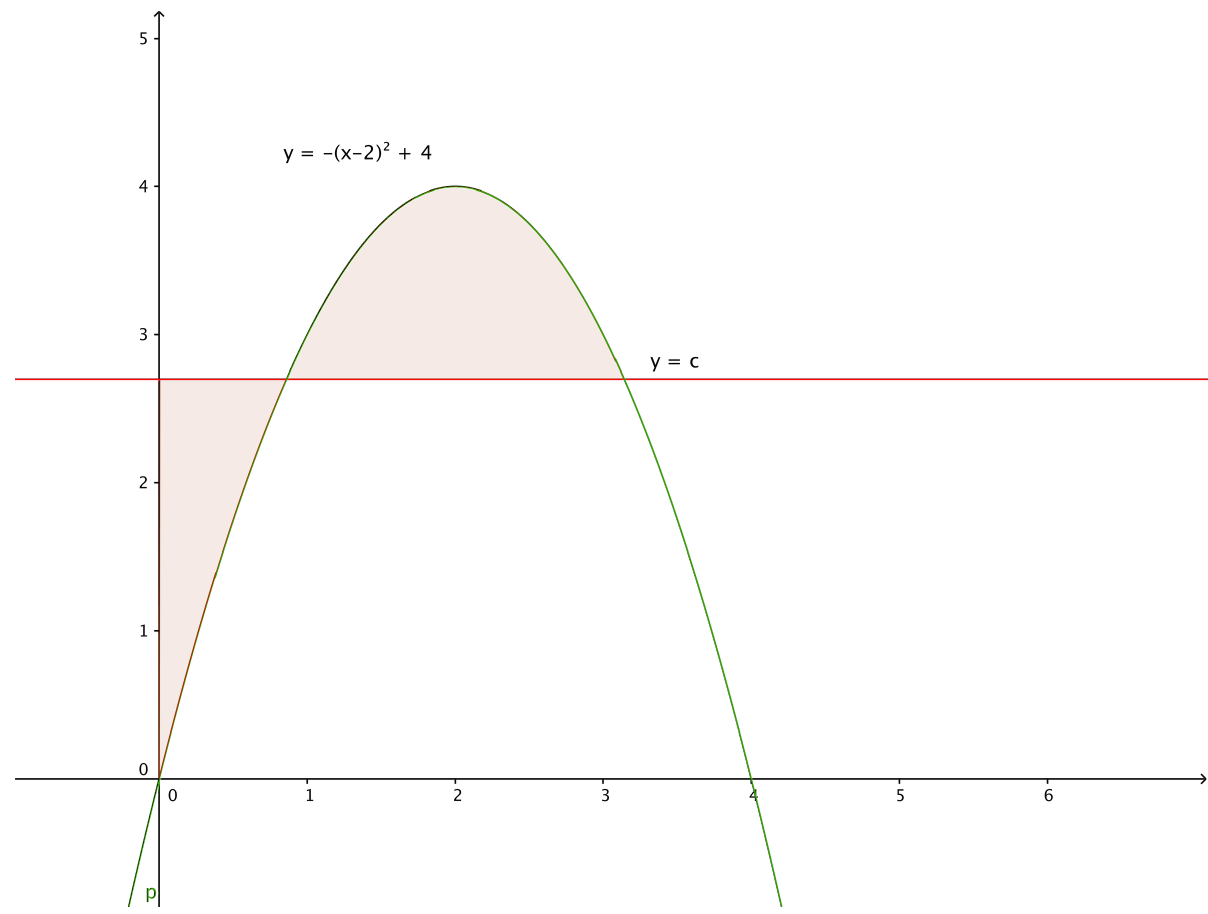
\includegraphics[width=1.2\textwidth]{seven.PNG}
\end{figure}	


\end{enumerate}

\end{document}
